
\documentclass{article}

\usepackage{graphviz}
\usepackage{url}
\usepackage{hyperref}
\usepackage{fullpage}
\usepackage{parskip}
\usepackage{fancyvrb}
\usepackage{amsmath}
\usepackage{framed}
\usepackage[section]{placeins}

\usepackage{listings}
\lstset{numbers=left,
		basicstyle=\footnotesize,
		captionpos=b,
		xleftmargin=0.3in}

\providecommand{\e}[1]{\ensuremath{\times 10^{#1}}}

\VerbatimFootnotes

\raggedright

% Change enumerate section numbering
\renewcommand*{\theenumii}{\theenumi.\arabic{enumii}}
\renewcommand*{\labelenumii}{\theenumi.\arabic{enumii}}

\begin{document}

% {{{ title page
\vspace*{1.0in}

\centerline{\LARGE \textbf{SprinklerPI}}
%\centerline{(Product Test Plan)}
\vspace{0.3in}
\centerline{\LARGE Product Test Plan}

\vfill

\begin{center}
\begin{tabular}{c}
Jeremiah Mahler \\
EECE 490B, CSU Chico \\
\today
\end{tabular}
\end{center}

\vspace{1in}

\thispagestyle{empty}

%\vfill

\pagebreak
% }}}

\thispagestyle{empty}
\tableofcontents
\clearpage

% {{{ Information Required for Execution
\section{Information Required for Execution}

\subsection{Purpose}

The purpose of this test protocol is to verify the full and complete
operation of the SprinklerPI system.

\subsection{Scope}

This test protocol should be executed to verify that each principal feature
and function performs within specification called out by the engineering
requirements document. In addition, other necessary specifications shall
be tested such as specific and necessary user, installation and power
requirements. The testing called out in this protocol is subject exclusively
to those selected specifications provided for the SprinklerPI.

\subsection{Responsibilities}

It is the responsibility of the assigned test engineer to execute all tests
included herein to the best of their ability. If necessary, seek additional
assistance to execute tasks.

\subsection{References}

Not applicable at this time.

%\subsection{Definitions}

\subsection{Equipment/Supplies}

\begin{itemize}
\item 110 volts AC power supply.
\item Digital volt meter.
\item Three test bridges (25 $\Omega$, 50 watt).
\item Ethernet network connection.
\item (optional) Wireless usb adapter.
\end{itemize}

\subsection{Precautions \& Warnings}

This test plan contains certain warnings, cautions and important
notes that the test engineer must be aware of while performing these tests.
The following illustrates each of these messages and how to recognize them.

\fbox{
\textbf{WARNING: \textless message\textgreater}
}

The ``WARNING: Message'' alerts the user about safety issues that are of
the highest importance, such as possible injury to the operator.

\fbox{
\textbf{CAUTION: \textless message\textgreater}
}

The ``CAUTION: Message'' alerts the user to issues concerning possible
damage to the equipment or that can lead to erroneous test results.

\fbox{
\textbf{IMPORTANT: \textless message\textgreater}
}

The ``IMPORTANT: Message'' alerts the user to important design changes.

% }}}

% {{{ Testing Features and Functions
\section{Testing Features and Functions}

This testing procedure can be used to determine if the system
is fully functional and operating within acceptable tolerances.

This is a minimal set of tests done at a high level of abstraction.
Low level sub-tests which provide no useful increase in the test scope
are not included.
In the event that a fault is found it is left up to an engineer to
determine the root cause.

Several assumptions are made in this test procedure.
It is assumed that networking has already been configured as
described in Appendix \ref{app:networking}.
It is also assumed that a fully populated SprinklerPI system with
three control/drivers is being tested.
This system is modular and the number of control/drivers can vary
from one to three.
Adapting these procedures to a reduced number of control/drivers should
be straightforward but this reduces the scope of the tests.

% {{{ Power On Test
\subsection{Power On Test}

\begin{enumerate}
\item Equipment Required
	\begin{itemize}
		\item 110 volts AC power outlet (NEMA 5-15R).
	\end{itemize}
\item Input
	\begin{itemize}
	\item (none)
	\end{itemize}
\item Output
	\begin{itemize}
	\item Green power LED on.
	\item Activity LEDs during boot up.
	\item Control LEDs off.
	\end{itemize}
\item Test Description \\

During power up the system should be seen going through several states
which can be seen by observing LED indicators (Figure \ref{fig:ledind}).
When it is complete it should end in a specific state.

After plugging the cord in to a 110 volt AC outlet the green LED on
the power supply should go on.
Then, as the computer boots up, activity should be seen on its LEDs.
The control LEDs may go on/off randomly as the system boots.
They also may may turn on valve number one during boot.
This is normal as the output pins go through random states and
is eventually cleared.
After approximately 30 seconds the activity LEDs on the computer
should reduce which indicates that the system has completed booting.
At this point all control/driver LEDs should be off.

\begin{figure}[hbp!]
% TODO - picture of fully populated system.
%      - label each of the LED indicators.
%      - group # on each control/driver
\caption{Location of LED indicators.}\label{fig:ledind}
\end{figure}

\pagebreak
\item Test Results \\
\vspace{1em}
\begin{tabular}{|l|l|l|l|}
	\hline
	\multicolumn{1}{|c|}{Test}
	& \multicolumn{1}{|c|}{Value}
	& \multicolumn{1}{|c|}{Pass/Fail}
	& \multicolumn{1}{|c|}{Notes} \\
	\hline
	Power LED on? & on / off && \hspace{1.7in} \\
	\hline
	Activity LEDs during boot? & yes / no && \\
	\hline
	Stable activity LEDs after boot up? & yes / no && \\
	\hline
	Control outputs off after boot up? & yes / no && \\
	\hline
\end{tabular}

\end{enumerate}
% }}}

% {{{ Manual Control Test
\clearpage
\subsection{Manual Control Test}
\label{sec:manual-control-test}

\begin{enumerate}
\item Equipment Required
	\begin{itemize}
	\item 110 volts AC power outlet (NEMA 5-15R).
	\item PC with Internet access and a web browser.
	\end{itemize}
\item Input
	\begin{itemize}
	\item User turns valves on using manual mode of web interface.
	\item User actuation of valves using manual mode of web interface.
	\end{itemize}
\item Output
	\begin{itemize}
	\item LED indicator for each valve which is turned on.
	\end{itemize}
\item Test Description \\

These tests verify that the valves can be manually operated from
the web interface (Figure \ref{fig:www-manual_mode}).
The user iterates through each possible combination and verifies
that the LED valve indicator is correct.

\begin{figure}[hbp!]
\begin{center}
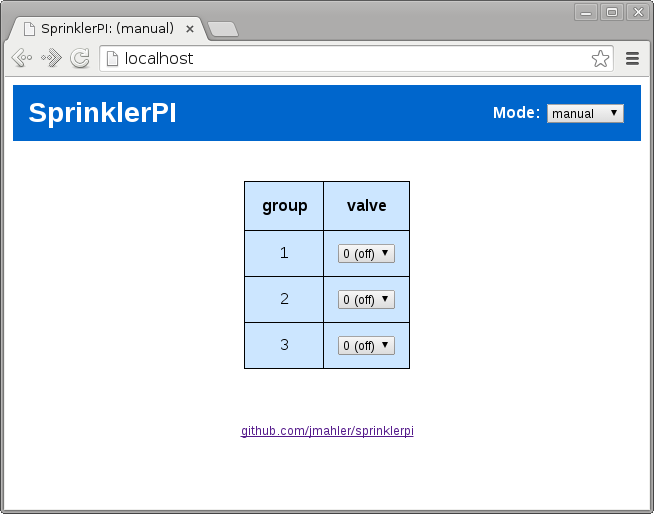
\includegraphics[scale=0.5]{img/www-manual_mode}
\end{center}
\caption{Web interface in manual mode which allows operation of
a single valve for each group.
The URL may be different depending on how the network is configured.}
\label{fig:www-manual_mode}
\end{figure}

It is assumed network has already been configured
(Appendix \ref{app:networking}) and that the URL of the server being
used for testing is known.

\pagebreak
\item Test Results \\
	\vspace{1em}
	\begin{tabular}{|c|c|c|c|c|}
		\hline
		Group & Valve & Value & Pass/Fail & Notes \\
		\hline
		1 & 0 & off && \hspace{20em} \\
		\hline
		1 & 1 & on && \\
		\hline
		1 & 2 & on && \\
		\hline
		1 & 3 & on && \\
		\hline
		1 & 4 & on && \\
		\hline
		1 & 5 & on && \\
		\hline
		1 & 6 & on && \\
		\hline
		1 & 7 & on && \\
		\hline
		1 & 8 & on && \\
		\hline
		\hline
		2 & 0 & off && \\
		\hline
		2 & 1 & on && \\
		\hline
		2 & 2 & on && \\
		\hline
		2 & 3 & on && \\
		\hline
		2 & 4 & on && \\
		\hline
		2 & 5 & on && \\
		\hline
		2 & 6 & on && \\
		\hline
		2 & 7 & on && \\
		\hline
		2 & 8 & on && \\
		\hline
		\hline
		3 & 0 & off && \\
		\hline
		3 & 1 & on && \\
		\hline
		3 & 2 & on && \\
		\hline
		3 & 3 & on && \\
		\hline
		3 & 4 & on && \\
		\hline
		3 & 5 & on && \\
		\hline
		3 & 6 & on && \\
		\hline
		3 & 7 & on && \\
		\hline
		3 & 8 & on && \\
		\hline
	\end{tabular}
\end{enumerate}
% }}}

% {{{ Power Supply Load Test
\clearpage
\subsection{Power Supply Load Test}

\begin{enumerate}
\item Equipment Required
	\begin{itemize}
	\item 110 volts AC power outlet (NEMA 5-15R).
	\item PC with Internet access and a web browser.
	\item Digital multi meter.
	\item Three control/Driver test bridges (25 $\Omega$, 5 Watt).
	\end{itemize}
\item Input
	\begin{itemize}
	\item 24 volts AC from 110 to 24 volts AC adapter.
	\item User actuation of valves using manual mode of web interface.
	\end{itemize}
\item Output
	\begin{itemize}
	\item $9.5\pm0.5$ volts AC across test bridge resistor when on.
	\item $24\pm4.8$ (20\%) volts AC output.
	\item $3.3\pm0.3$ (10\%) volts DC output.
	\end{itemize}
\item Test Description \\

This tests the power supply under a worst case load.
One test bridge is installed in each of the three control/drivers.
Then one valve on each group is turned on.
The voltage drop of the load in each test bridge is measured to
verify it is drawing a current.
Then the voltage output of the power supply is measured to verify
that it is adequitely supplying the load.

\begin{framed}
\textbf{IMPORTANT}: The DC voltage output of the power supply has
been changed from 5V to 3.3V.
The label on version 20140304 of the power supply PCB still
refers to 5V despite this change.
\end{framed}

\begin{figure}[hbp!]
% TODO - closeup of power supply with test points and orientation marked.
\begin{center}
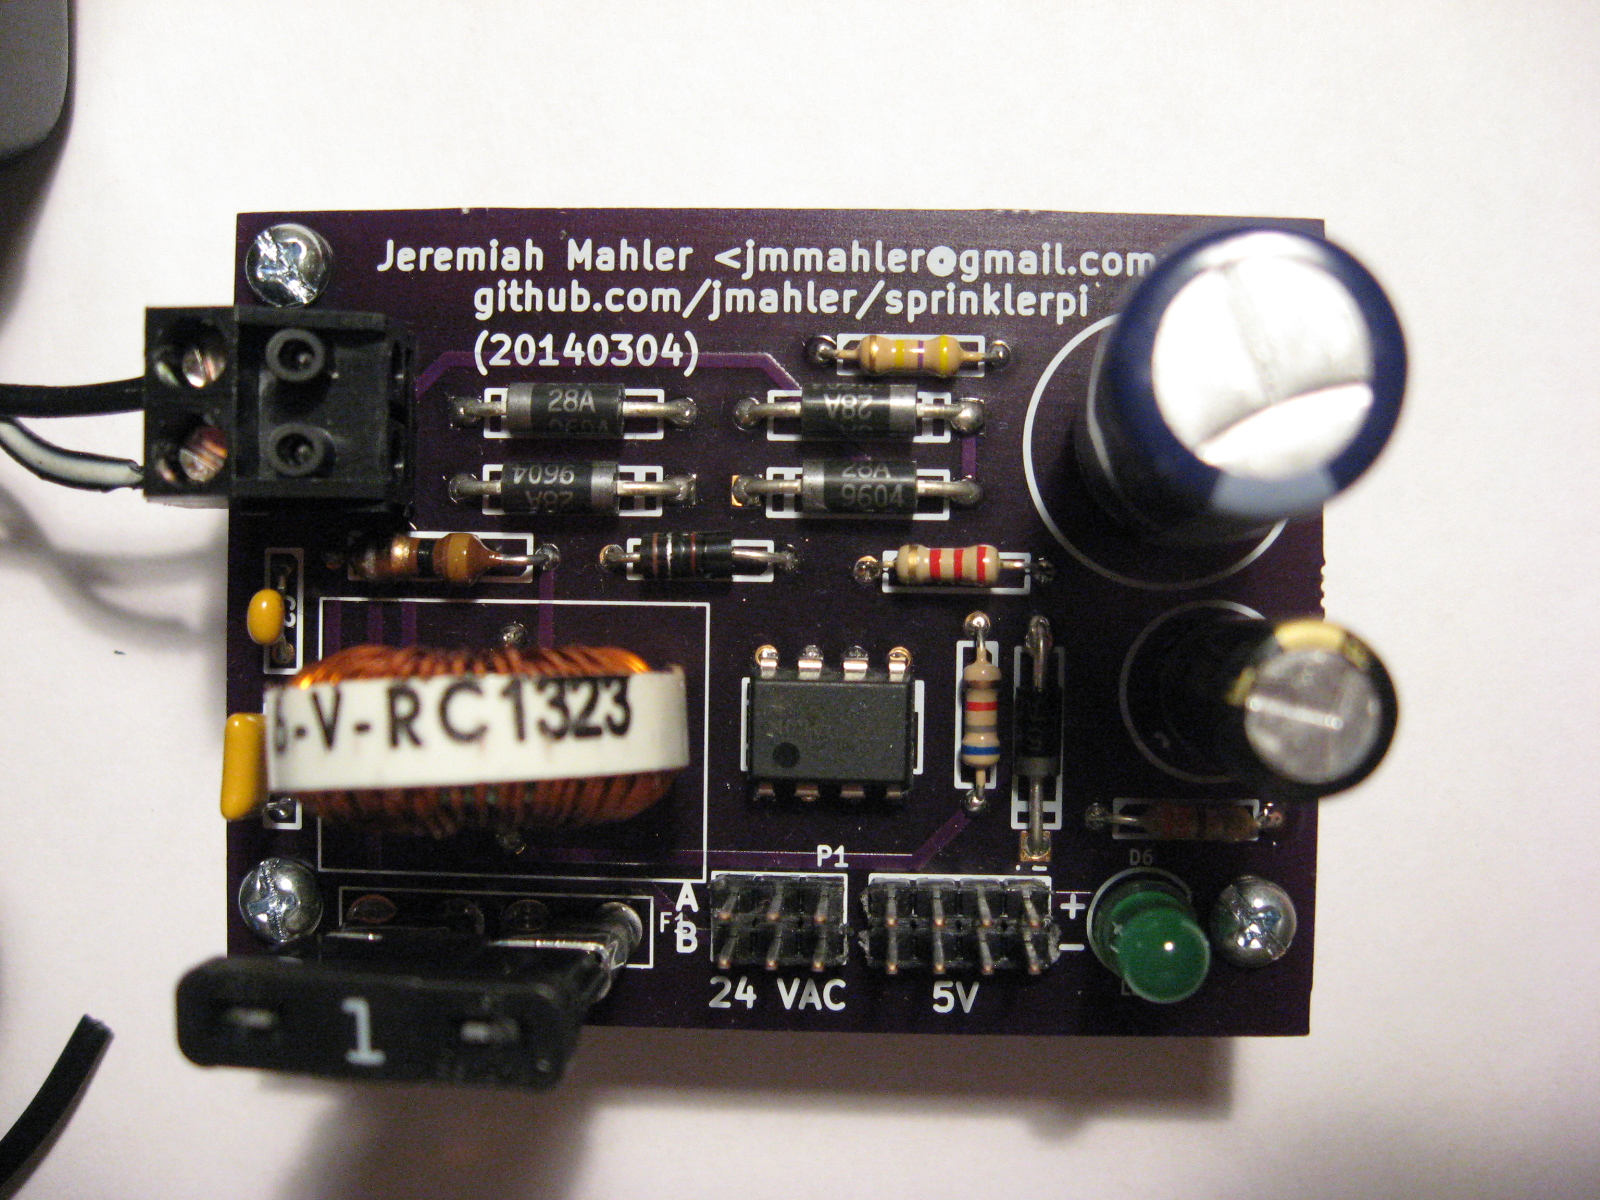
\includegraphics[scale=0.15,angle=0]{img/power_pcb-assembled-02.jpg}
\end{center}
\caption{Power supply test points for 3.3 volts DC and 24 volts AC.}
\label{fig:ps-test}
\end{figure}

\pagebreak

\item Test Results \\
	\vspace{1em}
	With three valves on, one in each group, the voltage drop
	across each test bridge load should be: $9.5\pm0.5$ VAC. \\
	\vspace{1em}
	\begin{tabular}{|c|c|c|c|c|}
		\hline
		Group & Valve	& Voltage Drop		& Pass/Fail & Notes \\
		\hline
		1 & 1 & & & \hspace{20em} \\
		\hline
		2 & 1 &&& \\
		\hline
		3 & 1 &&& \\
		\hline
	\end{tabular}

	\vspace{1em}
	With the three valves on, the power supply should provide
	$24\pm4.8$ volts AC and $3.3\pm0.3$ volts DC (Figure \ref{fig:ps-test}). \\
	\vspace{1em}
	\begin{tabular}{|c|c|c|c|}
		\hline
		Test  & Value & Pass/Fail & Notes \\
		\hline
		3.3 volts DC & & & \hspace{24em} \\
		\hline
		24 volts AC & & & \\
		\hline
	\end{tabular}

\end{enumerate}
% }}}

% {{{ Valve Load Test
\clearpage
\subsection{Valve Load Test}

\begin{enumerate}
\item Equipment Required
	\begin{itemize}
	\item 110 volts AC power outlet (NEMA 5-15R).
	\item PC with Internet access and a web browser.
	\item Digital multi meter.
	\item Three Control/Driver test bridges (25 $\Omega$, 5 Watt).
	\end{itemize}
\item Input
	\begin{itemize}
	\item User actuation of valves using manual mode of web interface.
	\end{itemize}
\item Output
	\begin{itemize}
	\item $9.5\pm0.5$ volts AC across test bridge resistor when on.
	\end{itemize}

\pagebreak
\item Test Description \\

In this test the valves connected to a test bridge which will place
a load on the circuit when the valve is on.
Then the valves are manually operated from the web interface and
the voltage drop across the load is measured.
Additionally, the output voltages of the power supply are measure
when under load to verify that they are operating within an acceptable range.

\begin{framed}
\textbf{IMPORTANT}: The DC voltage output of the power supply has
been changed from 5V to 3.3V.
The label on version 20140304 of the power supply PCB still
refers to 5V despite this change.
\end{framed}

\item Test Results \\
	\vspace{1em}
	One valve should be on in each group during the entire test
	to ensure the worst case load.
	The voltage drop across the test bridge load should be: $9.5\pm0.5$ VAC. \\
	\vspace{1em}

	\begin{tabular}{|c|c|c|c|c|}
		\hline
		Group & Valve & Voltage Drop & Pass/Fail & Notes \\
		\hline
		1 & 1 &  && \hspace{20em} \\
		\hline
		1 & 2 &  && \\
		\hline
		1 & 3 &  && \\
		\hline
		1 & 4 &  && \\
		\hline
		1 & 5 &  && \\
		\hline
		1 & 6 &  && \\
		\hline
		1 & 7 &  && \\
		\hline
		1 & 8 &  && \\
		\hline
		\hline
		2 & 1 &  && \\
		\hline
		2 & 2 &  && \\
		\hline
		2 & 3 &  && \\
		\hline
		2 & 4 &  && \\
		\hline
		2 & 5 &  && \\
		\hline
		2 & 6 &  && \\
		\hline
		2 & 7 &  && \\
		\hline
		2 & 8 &  && \\
		\hline
		\hline
		3 & 1 &  && \\
		\hline
		3 & 2 &  && \\
		\hline
		3 & 3 &  && \\
		\hline
		3 & 4 &  && \\
		\hline
		3 & 5 &  && \\
		\hline
		3 & 6 &  && \\
		\hline
		3 & 7 &  && \\
		\hline
		3 & 8 &  && \\
		\hline
	\end{tabular}

\end{enumerate}
% }}}

% {{{ Scheduler Queuing Test
\clearpage
\subsection{Scheduler Queuing Test}

\begin{enumerate}
\item Equipment Required
	\begin{itemize}
	\item 110 volts AC power outlet (NEMA 5-15R).
	\item Computer with web browser and network connection.
	\end{itemize}
\item Input
	\begin{itemize}
	\item Schedule time and duration to run valve.
	\end{itemize}
\item Output
	\begin{itemize}
	\item Valves go on and runs for the expected amount of time.
	\end{itemize}

\item Test Description \\

This tests the scheduler queuing mechanism by starting multiple
operations in one group simultaneously.
Each operation should be completed and run for the expected amount
of time although the order of operations is not guaranteed.

The LED valve indicators can be used to determine when the valve is on.

\pagebreak
\item Test Results \\
	\vspace{1em}
	For a single group configure it to start three different valves
	at the same start time as shown in Figure \ref{fig:www-schedule_test1}.
	The start time should be adjusted to some future time relative
	to a particular local time.
	The run time can be any small amount such as 30 seconds. \\

	\begin{figure}[hbp!]
	\begin{center}
	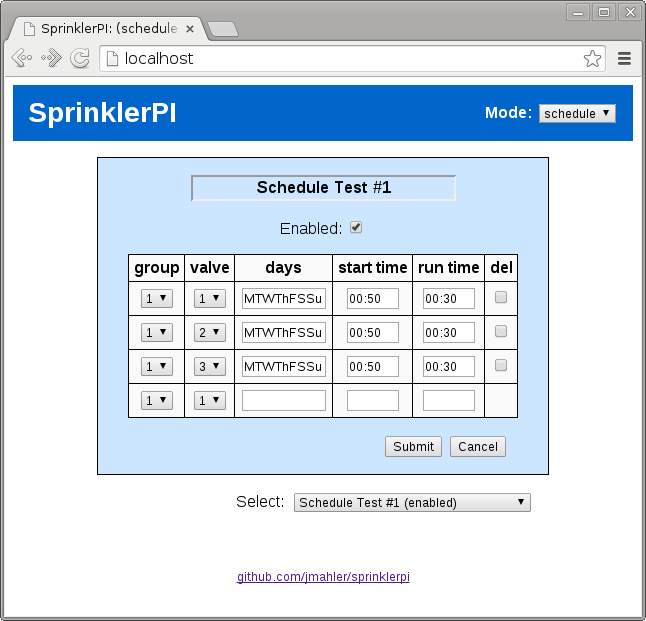
\includegraphics[scale=0.5]{img/www-schedule_test1}
	\end{center}
	\caption{Schedule configured to start three valves in one group
		simultaneously.}
	\label{fig:www-schedule_test1}
	\end{figure}

	\vspace{1em}
	\begin{center}
	\begin{tabular}{|c|c|c|c|c|c|c|}
		\hline
		Group & Valve & Start Time & Run Time & Stop Time & Duration & Pass/Fail \\
		\hline
		1 & 1 & & 00:30 & & & \hspace{4em} \\
		\hline
		1 & 2 & (same) & 00:30 & & & \\
		\hline
		1 & 3 & (same) & 00:30 & & & \\
		\hline
		\hline
		\multicolumn{7}{|c|}{Notes} \\
		\multicolumn{7}{|c|}{} \\
		\multicolumn{7}{|c|}{} \\
		\multicolumn{7}{|c|}{} \\
		\multicolumn{7}{|c|}{} \\
		\hline
	\end{tabular}
	\end{center}

\end{enumerate}

% }}}

% {{{ Scheduler Concurrency Test
\clearpage
\subsection{Scheduler Concurrency Test}

\begin{enumerate}
\item Equipment Required
	\begin{itemize}
	\item 110 volts AC power outlet (NEMA 5-15R).
	\item Computer with web browser and network connection.
	\end{itemize}
\item Input
	\begin{itemize}
	\item Schedule time and duration to run valve.
	\end{itemize}
\item Output
	\begin{itemize}
	\item Valves go on and runs for the expected amount of time.
	\end{itemize}

\item Test Description \\

This tests the scheduler queuing mechanism by starting
operations in different groups simultaneously.
Each operation should be completed and run for the expected amount.
They should run concurrently since they are in different groups.

The LED valve indicators can be used to determine when the valve is on.

\pagebreak
\item Test Results \\
	\vspace{1em}
	For different groups configure it to start a valve 
	at the same time as shown in Figure \ref{fig:www-schedule_test2}.
	The start time should be adjusted to some future time relative
	to a particular local time.
	The run time can be any small amount such as 30 seconds. \\

	\begin{figure}[hbp!]
	\begin{center}
	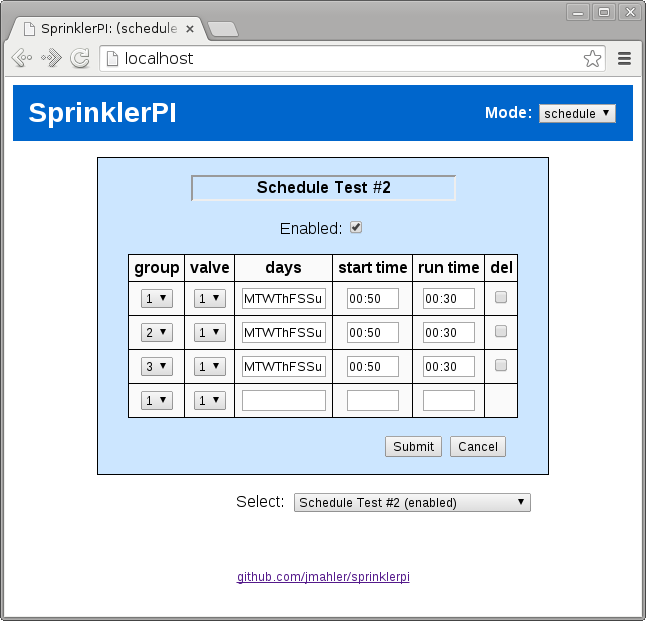
\includegraphics[scale=0.5]{img/www-schedule_test2}
	\end{center}
	\caption{Schedule configured to start three valves in different groups
		simultaneously.}
	\label{fig:www-schedule_test2}
	\end{figure}

	\vspace{1em}
	\begin{center}
	\begin{tabular}{|c|c|c|c|c|c|c|}
		\hline
		Group & Valve & Start Time & Run Time & Stop Time & Duration & Pass/Fail \\
		\hline
		1 & 1 & & 00:30 & & & \hspace{4em} \\
		\hline
		2 & 1 & (same) & 00:30 & & & \\
		\hline
		3 & 1 & (same) & 00:30 & & & \\
		\hline
		\hline
		\multicolumn{7}{|c|}{Notes} \\
		\multicolumn{7}{|c|}{} \\
		\multicolumn{7}{|c|}{} \\
		\multicolumn{7}{|c|}{} \\
		\multicolumn{7}{|c|}{} \\
		\hline
	\end{tabular}
	\end{center}

\end{enumerate}

\FloatBarrier
% }}}

% }}}

\clearpage
\appendix

% {{{ Network Configuration
\section{Network Configuration}
\label{app:networking}

% TODO

% }}}

\end{document}

